\section{$\R$上的勒贝格外测度与测度的构造}
\subsection{正课内容总结}

在正课中, 我们首先从区间这一类$\R$中最简单的集合出发, 定义了有界区间的\textbf{长度}. 若$a,b \in \R, a < b$, 则定义
$(a,b), [a,b], (a,b], [a,b)$的\textbf{长度}均为$b-a$, 即
$$|(a,b)| = |[a,b]| = |(a,b]| = |[a,b)| = b-a. $$
接着我们利用下确界定义了所有集合的勒贝格外测度, 再使用Carath\'eorody条件加以限制, 得到了$\calP(\R)$的一个真子族: 勒贝格可测集构成的集族. 
我们以开区间构成定理为基础, 利用开区间覆盖以及下确界定义了$\R$上的勒贝格外测度, 再利用\textbf{Carath\'eodory条件}加以限制得到勒贝格测度. 勒贝格测度$m$满足以下性质:
\begin{enumerate}
    \item  $m(\varnothing) = 0$;
    \item (可数可加性)若$\{E_n\}$是一列互不相交的可测集, 则
    $$m\br{\bCup{n=1}{\infty}E_n} = \Sum{n=1}{\infty}m(E_n).$$
\end{enumerate}
可测集族满足以下性质:
\begin{enumerate}
    \item 空集和$\R^n$可测;
    \item 若$\{E_n\}$是一列可测集, 则$\bCup{n=1}{\infty}E_n$可测;
    \item 若$E$可测, 则$E^c$可测.
\end{enumerate}
由此我们得到了$\R$上的一种集合-代数结构: 勒贝格$\sigma$-代数. 我们可以将勒贝格测度与勒贝格$\sigma$-代数推广至一般的集合. 
$m$做了哪些事? 输入一个可测集$E$, $m(E)$便返回一个值, 该值属于$[0,\infty]$ (注意$\infty$可以取到, 例如$m(\R) = \infty$). 
于是得到元素间的对应关系$E \mapsto m(E)$. 
\begin{exercise}
    找出$m$的定义域与值域, 将$m$这个映射写成标准形式. 
\end{exercise}
设$X$是一个集合, $\calM$是$X$的一些子集构成的集族. 如果$\{E_n\}_{n=1}^\infty \subset \calM \implies \bCup{n=1}{\infty}E_n \in \calM$且$E \in \calM \implies E^c \in \calM$, 则称$\calM$为$X$上的一个$\sigma$-代数, $\calM$中的元素称为\textbf{可测集}. 
而抽象测度正是定义在$\calM$上的一个可数可加的函数: 设$\mu: \calM \to [0, \infty]$, 如果$\mu$满足
\begin{enumerate}
    \item $\mu(\varnothing) = 0$;
    \item 若$\{E_n\}$是一列互不相交的可测集, 则
    $$\mu\br{\bCup{n=1}{\infty}E_n} = \Sum{n=1}{\infty}\mu(E_n),$$
\end{enumerate}
那么称$\mu$为$\calM$上的一个\textbf{测度}.

不难发现, 体积和外测度实际上也是定义在某些集族上的函数:
体积\footnote{这里直接当成日常生活中(推广至$d$维)的体积即可, 并且仅定义在方体, 矩体上}定义在方体构成的集族上, 外测度定义在所有幂集上, 测度定义在$\sigma$-代数上.
现在我们从上节的构造过程归纳出重要步骤, 厘清如何从简单到复杂. 
我们不妨以勒贝格测度为例列一张表格:
\begin{center}
    \begin{tabular}{ |c|c|c|c| } 
    \hline
    函数 & 对应的``图形" & 对应的集族(定义域) & 如何得到 \\ 
    \hline
    体积 & 开区间 & 所有开区间构成的集族$\calQ$  & 生活经验 \\ 
    \hline
    外测度 & 任一子集 & 幂集$\calP(\R^n)$ & 可数多个开区间的覆盖取下确界 \\ 
    \hline
    测度 & 可测集 & Lebesgue $\sigma$-代数$\calL$ & Carath\'eodory条件 \\
    \hline
    \end{tabular}
\end{center}
先从最基本的具有先验体积的图形\footnote{大家可以直接想象成方体}出发(building block), 我们手头上就有了一个定义在$\calQ$上的体积函数$\rho$, 且这个函数自然地满足有限可加性(有限多个不交的区间的体积等于各自体积之和). 接着用可数多个区间覆盖任一集合, 对这些区间体积和取下确界得到定义在$\calP(\R^n)$上的函数: 外测度$m^*$. 最后, 用某些条件去限制一个集合满足关于$m^*$的某个不等式, 从而缩小$\calP(\R^n)$的范围, 得到可测集类, 同时也是个$\sigma$-代数.\footnote{如果感到这段话难以理解, 请学习正课对应的内容}

在抽象测度论中我们将会学习如何构造一个测度, 也是从简单到复杂, 分为4个步骤\footnote{此处为预告, 不需要掌握. 半代数和代数也是类似于$\sigma$-代数的一种结构}:
\begin{center}
    (体积, 半代数) $\rightarrow$ (预测度, 代数) $\rightarrow$ (外测度, 幂集) $\rightarrow$ (测度, $\sigma$-代数)
\end{center}
相信大家在学习抽象测度论时, 不会感到陌生. 

最后, 我们再了解一下外测度的公理化定义(外测度在实际应用中基本都是基本图形覆盖+下确界这一套组合, 很少出现纯种的抽象外测度). 总结一下勒贝格外测度的性质, 我们将其推广至一般的集合$X$. 
若$\mu^*: \calP(X) \to [0, \infty]$满足
\begin{enumerate}
    \item $\mu^*(\varnothing) = 0$;
    \item $A \subset B \implies \mu^*(A) \leq \mu^*(B)$;
    \item $\mu^*\br{\bCup{n=1}{\infty}A_n} \leq \Sum{n=1}{\infty} \mu^*(A_n)$,
\end{enumerate}
则称$\mu^*$为$X$上的一个外测度. 

\begin{exercise}
    设$\mu^*$是$X$上的一个外测度.
    设$B \subset X$. 定义$\mu_B: \calP(X) \to [0, \infty]$如下:
    $$\mu_B(A) = \mu^*(A \cap B).$$
    验证: $\mu_B$也是$X$上的一个外测度. 
\end{exercise}
\begin{proof}
    显然$\mu_B(\varnothing) = 0$. 设$E \subset F$, 则
    $E \cap B \subset F \cap B$, 所以$\mu^*(E \cap B) \leq \mu^*(F \cap B)$, 即$\mu_B(E) \leq \mu_B(F)$. 设$\{E_n\}_{n=1}^\infty$为$X$中的一列集合, 则$\mu_B\br{\bCup{n=1}{\infty}E_n} = \mu^*\br{ \br{\bCup{n=1}{\infty}E_n} \cap B}$.
    因为$\bCup{n=1}{\infty}E_n \cap B = \bCup{n=1}{\infty}(E_n \cap B)$, 所以利用$\mu^*$已经是外测度这一条件得
    $$\mu_B\br{\bCup{n=1}{\infty}E_n} = \mu^*\br{\bCup{n=1}{\infty}(E_n \cap B)} \leq \Sum{n=1}{\infty} \mu^*(E_n \cap B) = \Sum{n=1}{\infty} \mu_B(E_n). $$
    \qed 
\end{proof}
\begin{exercise} % Stein 1-26
    设$A \subset E \subset B$, $A,B$具有有限测度. 证明: 若$m(A) = m(B)$, 则$E$可测.
\end{exercise}
\begin{proof}
    因为$m(E \setminus A) \leq m(B \setminus A) = m(B) - m(A) = 0$, 所以$E \setminus A$可测, 
    从而$E = A \cup (E \setminus A)$可测. \qed 
\end{proof}


\subsection{其他外测度限制条件}
阅读过不止一本实分析教材的同学可能会发现, 在限制外测度的定义域时, 除了用Carath\'eodory条件, 还有别的限制方式. Stein的\textit{Real Analysis}是这样定义可测集的:
设$E$是一个集合, 若对任意$\eps > 0$都存在一个开集$U \supset E$, 使得$m^*(U \setminus E) < \eps$, 则称$E$为(勒贝格)可测集. 这种定义方式更符合几何直觉: 如果一个开集能够``较好地"盖住集合$E$, 那么$E$就是可测的, 且定义勒贝格测度$m(E) = m^*(E)$. 从该定义出发, 我们同样能够证明可测集类的封闭性以及$m$的可数可加性, 这里以并集为例:
\begin{example}
    利用另一种可测集的定义, 证明: 设$\{E_n\}_{n=1}^\infty$为一列可测集, 则$\bCup{n=1}{\infty}E_n$可测.
\end{example}
\begin{proof}
    首先, 对每个$n \in \N$都存在$U_n$使$m^*(U_n \setminus E_n) < 2^{-n} \eps$.
    显然$\bCup{n=1}{\infty}U_n \supset \bCup{n=1}{\infty}E_n$, 且
    $\bCup{n=1}{\infty}U_n \setminus \bCup{n=1}{\infty}E_n = \bCup{n=1}{\infty} (U_n \setminus E_n)$, 所以
    $$  m^*\br{\bCup{n=1}{\infty}U_n \setminus \bCup{n=1}{\infty}E_n}
    \leq \Sum{n=1}{\infty}m^*\br{U_n \setminus E_n} < \eps. $$
    \qed 
\end{proof}
在``开集逼近"这一定义下, 大部分可测集的性质证明都是传统的$\eps$方法, 而在Carath\'eodory条件的框架下, 证明则更多的是一路等于号的代数变形. 

我们现在来聊聊更深层次的区别: 
Carath\'eodory条件是一个等式, 而且对任意集合都能用. 开集逼近条件则要求我们的原始集合上要具备一个拓扑(开集是拓扑中的元素). 当然在$\R$中这个差别体现不出来, 但当我们要在更一般的集合$X$上构造测度时, 几乎就只能采用Carath\'eodory条件, 因为它只涉及到代数运算. 我们在学习抽象测度构造方法论时, 还会再见到Carath\'eodory条件. 

最后, 你一定想问: 这两种定义等价吗? 这里我们需要借助勒贝格测度的\textbf{正则性质}. 从开集逼近定义出发, 对每个$n \in \N$我们都能找到$U_n \supset E$满足$m^*(U_n \setminus E) < 1/n$, 令$U = \bCap{n=1}{\infty}U_n$, 则$m^*(U \setminus E) = 0$, 于是$E = U \setminus (U \setminus E)$具有$G_\delta \setminus$(0测集)的形式, 所以$E$可测, 自然满足Carath\'eodory条件. 反过来, 正课中我们从Carath\'eodory条件出发推得的一条正则性质($\forall \eps>0~\exists$开集$U \supset E: m^*(U \setminus E)<\eps$)正是开集逼近条件.

\begin{remark}
    为保证行文连贯, 我在讲义写正则性质与测度的极限运算之前用到了这些结果, 如读者在这里对它们感到陌生, 请调整阅读顺序. 
\end{remark}




\subsection{无交化处理与Venn图}
实分析会牵涉到大量的集合运算, 与此同时我们还要估计这些集合的测度. 
由于测度对互不相交的集合列具有可数可加性, 在应用中我们常常要想方设法将一个集合写成无交并的形式, 例如
$$E \cup F = (E \setminus F) \cup (E \cap F) \cup (F \setminus E) = (E \Delta F) \cup (E \cap F).$$
这个式子在集合论上虽然正确, 但是对测度论却没有什么价值, 因为$\mu(E \setminus F)$并不一定等于$\mu(E) - \mu(F)$: 我们减得太``多"了.
$E$可以写成无交并$$E=(E \setminus (E \cap F)) \cup (E \cap F),$$ 
$F$可以写成无交并$$F=(F \setminus (E \cap F)) \cup (E \cap F),$$
从而
$$E \cup F = (E \setminus (E \cap F)) \cup (E \cap F) \cup (F \setminus (E \cap F)). $$

\begin{exercise}
    假设上面出现的集合均可测(一般的可测), 将测度$\mu$套到等号两边, 写出测度作用与集合运算的恒等式. 
\end{exercise}
% 在解答中穿插Venn图的应用
\begin{exercise}\label{inclu-exclu-basic-case}
    设$E,F \subset X$为可测集, 则$\mu(E)+\mu(F) = \mu(E \cup F) + \mu(E \cap F)$.
\end{exercise}
\begin{proof}
    若$E$和$F$的其中一个测度为$\infty$, 则显然$\infty = \infty$. 现设$\mu(E)<\infty, \mu(F)<\infty$ (想做减法, 就必须保证有限, 因为$\infty - \infty$没有定义, 所以不能出现这种样子的表达式). \\
    记$A = E \cap F$, 则
    \begin{align*}
    %\mu(E \cup F)
    %&= \mu(E \cup (F \setminus A)) = \mu(E) + \mu(F \setminus A), \\
    \mu(E \cup F)
    &= \mu(F \cup (E \setminus A)) = \mu(F) + \mu(E \setminus A) \\
    \mu(E) &= \mu((E \setminus A) \cup A)
    = \mu(E \setminus A) + \mu(E \cap F). 
    \end{align*}
    两式相减得结论. \qed 
\end{proof}
\begin{remark}
    从直觉上看, 将$E$的测度和$F$的测度相加, 则会多加一次$E \cap F$的测度, 所以要将其减去, 这样就有
    $\mu(E \cup F) = \mu(E) + \mu(F) - \mu(E \cap F)$. 
\end{remark}
\begin{example}
    设$E,F \subset X$为可测集. 
    \begin{enumerate}
    \item 若$\mu(E \Delta F) = 0$, 则$\mu(E)=\mu(F)$. ($E \Delta F = (E \setminus F) \cup (F \setminus E)$).
    \item 若$\mu(E \Delta F) = 0$, 则称$E \sim F$. 证明$\sim$是$\sigma$-代数$\calM$上的一个等价关系. 
    \end{enumerate}
\end{example}
\begin{proof}
    \begin{enumerate}
    \item 我们并不能直接把测度套用在$E \Delta F$的原始定义上, 因为$\mu(E \setminus F)$一般不等于$\mu(E)-\mu(F)$. 记$A=E \cap F$, 则
    $$E \Delta F = (E \setminus A) \cup (F \setminus A), $$
    所以$\mu(E \Delta F) = \mu(E \setminus A) + \mu(F \setminus A) = 0$, 从而
    $\mu(E \setminus A) = \mu(F \setminus A) = 0$.
    于是
    \begin{align*}
        &\mu(E) = \mu(E \setminus A) + \mu(A) = \mu(A), \\
        &\mu(F) = \mu(F \setminus A) + \mu(A) = \mu(A).
    \end{align*}
    \item 显然$\mu(E \Delta E) = 0$. 若$\mu(E \Delta F) = 0$, 则$\mu(F \Delta E) = \mu(E \Delta F) = 0$. 现设$E \sim F, F \sim G$, 则$\mu(E \Delta F) = \mu(F \Delta G) = 0$, 想要证$\mu(E \Delta G) = 0$. 
    我们的思路自然是将$E\Delta G$写成无交并: 先画出$E, F, G$的Venn图, 写出每一个交集, 最后代入$E \Delta G$.
    \begin{figure}[h]
        \centering
        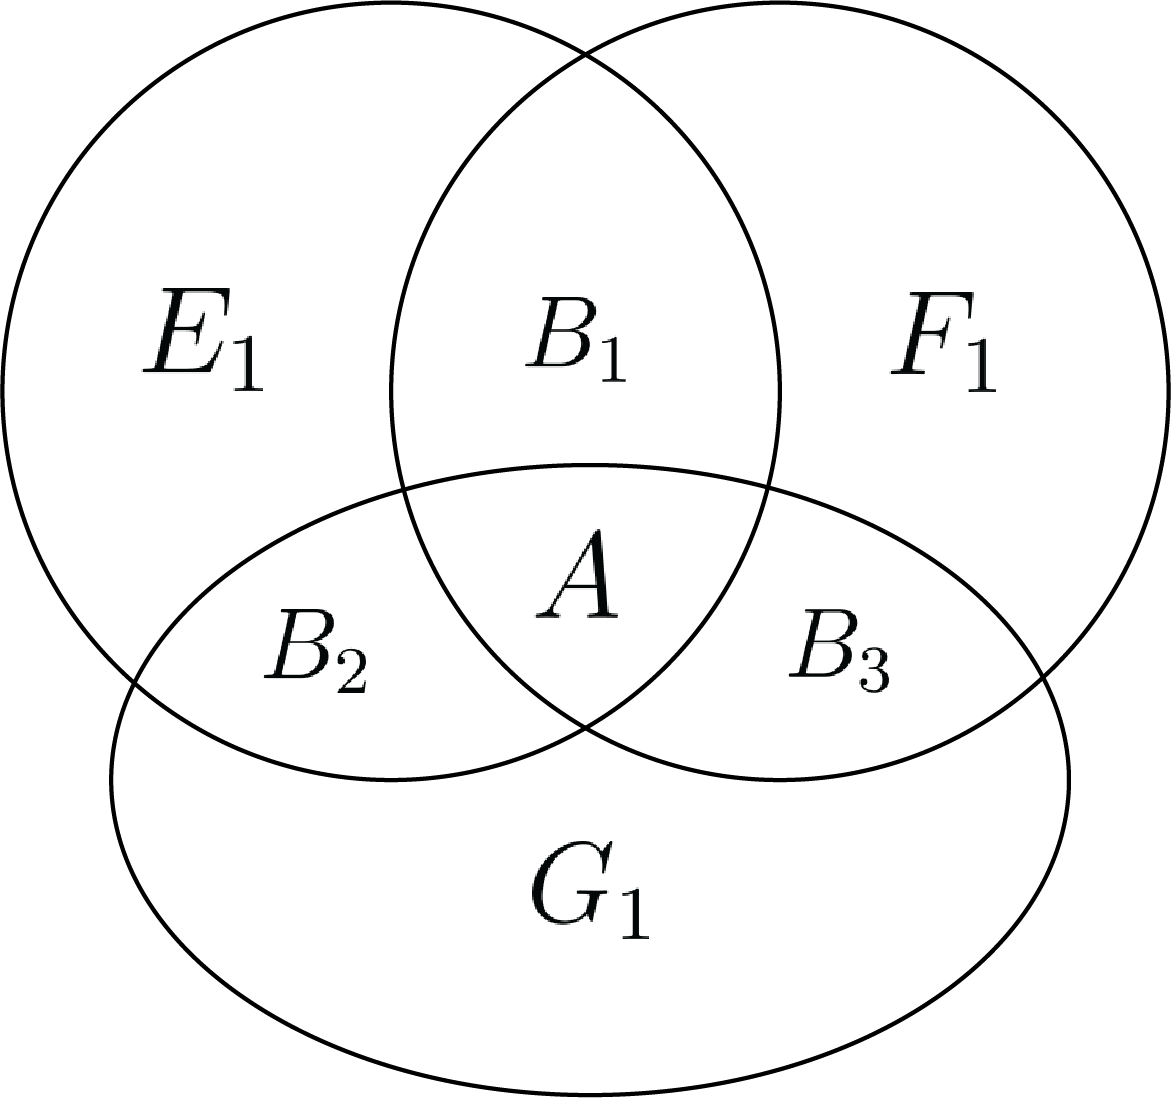
\includegraphics[scale=0.6]{figure/Venn_1.png}
        %\caption{Caption}
    \end{figure}
    
    令
    \begin{align*}
        &A = E \cap F \cap G, \\
        &B_1 = (E \cap F) \setminus A, \quad B_2 = (E \cap G) \setminus A, \quad B_3 = (F \cap G) \setminus A, \\
        &E_1 = E \setminus (B_1 \cup B_2 \cup A), \quad
         F_1 = F \setminus (B_1 \cup B_3 \cup A), \quad
         G_1 = G \setminus (B_2 \cup B_3 \cup A).
    \end{align*}
    则由条件知
    \begin{align*}
        &\mu(E_1 \cup B_2) + \mu(F_1 \cup B_3) = \mu(E_1)+\mu(B_2)+\mu(F_1)+\mu(B_3)=0, \\
        &\mu(F_1 \cup B_1) + \mu(G_1 \cup B_2) = \mu(F_1)+\mu(B_1)+\mu(G_1)+\mu(B_2)=0,
    \end{align*}
    则
    $$\mu(E \Delta G)
    = \mu(E_1 \cup B_1)+\mu(G_1 \cup B_3) 
    = \mu(E_1) + \mu(B_1) + \mu(G_1) + \mu(B_3) = 0. $$
    \end{enumerate}
    \qed 
\end{proof}
\begin{example}[~容斥原理(inclusion–exclusion principle)]
    现在我们介绍概率论中常用的\textbf{容斥原理}. 为此, 我们先引入概率测度$\P$. 设$(X, \calF, \P)$为一测度空间, 如果测度$\P$满足$\P(X) = 1$, 则称$(X,\calF,\P)$为一个\textbf{概率空间}(probability space), $\P$为其上的一个\textbf{概率测度}(probability measure), 简称概率. 令练习 \ref{inclu-exclu-basic-case} 中的$\mu$为概率测度$\P$可得两个集合的容斥原理
    $$\P(E \cup F) = \P(E)+\P(F) - \P(E \cap F). $$
    再次利用上一个例子中的Venn图, 我们有
    \begin{align*}
        E \cup F \cup G
        &= E \cup F_1 \cup B_3 \cup G_1 \\
        &= E \cup (F \setminus (A \cup B_1)) \cup (G \setminus (B_2 \cup B_3 \cup A)) \\
        &= E \cup (F \setminus (E \cap F)) \cup (G \setminus (B_2 \cup B_3 \cup A)), 
    \end{align*}
    则
    \begin{align*}
        \P(E \cup F \cup G)
        &= \P(E) + \P(F) - \P(E \cap F) + \P(G) - \P(B_2 \cup B_3 \cup A) \\
        &= \P(E)+\P(F)+\P(G) - \P(E \cap F) - [\P( (B_2 \cup A) \cup (B_3 \cup A) )] \\
        &= \P(E)+\P(F)+\P(G) - \P(E \cap F) - [\P( (B_2 \cup A) + \P(B_3 \cup A) - \P(A)] \\
        &= \P(E)+\P(F)+\P(G) - \P(E \cap F) - \P(E \cap G) - \P(F \cap G) + \P(E \cap F \cap G).
    \end{align*}
    但是对$n$个集合的情形, 我们就不能画Venn图了, 需要用数学归纳法. 一般地, 设$A_1, \cdots, A_n \in \calF$, 则
    \begin{equation}
    \P\br{\bCup{i=1}{n}A_i}
    = \Sum{i=1}{n}\P(A_i) - \sum_{i<j}\P(A_i \cap A_j) 
    + \sum_{i<j<k}\P(A_i \cap A_j \cap A_k) + \cdots + 
    (-1)^{n-1}\P\br{\bCap{i=1}{n}A_i}.
    \end{equation}
\end{example}
\begin{proof}
    假设容斥原理对$n$成立, 我们只需证明它对$n+1$也成立. 
    因为$\bCup{i=1}{n+1}A_i = \bCup{i=1}{n}A_i \cup A_{n+1}$, 所以我们可以套用$n=2$的容斥原理, 得
    $$\P\br{\bCup{i=1}{n}A_i \cup A_{n+1}}
    = \P\br{\bCup{i=1}{n}A_i} + \P(A_{n+1}) - \P\br{\bCup{i=1}{n}A_i \cap A_{n+1}}. $$
    这样右边最多就只有$n$个集合的并, 所以由归纳假设得
    \begin{align*}
    \P\br{\bCup{i=1}{n}A_i \cap A_{n+1}}
    &= \R\br{\bCup{i=1}{n} (A_i \cap A_{n+1})} \\
    &= \Sum{i=1}{n}\P(A_i \cap A_{n+1}) - \sum_{i<j \leq n}\P(A_i \cap A_j \cap A_{n+1}) 
    + \cdots + 
    (-1)^{n-1}\P\br{A_1 \cap \cdots \cap A_n \cap A_{n+1}},
    \end{align*}
    还有
    \begin{align*}
    \P\br{\bCup{i=1}{n}A_i}
    = \Sum{i=1}{n}\P(A_i) - \sum_{i<j \leq n}\P(A_i \cap A_j) 
    + \cdots + (-1)^{n-1}\P\br{A_1 \cap \cdots \cap A_n}.
    \end{align*}
    将上面两式相加, 得
    \begin{align*}
    \P\br{\bCup{i=1}{n}A_i \cup A_{n+1}}
    &= \Sum{i=1}{n+1}\P(A_i) - \sum_{i<j\leq n+1}\P(A_i \cap A_j)
    + \cdots \\
    &\quad + (-1)^{n-1}[\P(A_1 \cap \cdots \cap A_{n-1} \cap A_n) + 
                        \P(A_1 \cap \cdots \cap A_{n-1} \cap A_{n+1})] \\
    &\quad + (-1)^n \P(A_1 \cap \cdots \cap A_{n+1}),
    \end{align*}
    故容斥原理对$n+1$也成立, 所以对所有$n \in \N^+$都成立. \qed 
\end{proof}

%在利用Carath\'eodory条件证明勒贝格可测集对交, 并, 补的封闭性时,  也用到了这一思想. 
\subsection{Carath\'eodory条件中试验集的选取}
设$A \subset \R$, 若对任意集合$E \subset \R$, 有
\begin{equation}
    m^*(E) = m^*(E \cap A) + m^*(E \cap A^c), 
\end{equation}
则称$A$为勒贝格可测集, 而$E$一般可叫作\textbf{试验集}. 许多关于集合可测性结论的证明, 都依赖于试验集的巧取. 
\begin{exercise}[~(复习)]
    设$m^*$是$\R$上的勒贝格外测度, $A,B$为勒贝格可测集, 证明$A \cup B$也是勒贝格可测集. 
\end{exercise}
\begin{proof}
    设$E \subset \R$, 则
    \begin{align*}
    m^*(E) &= m^*(E \cap A) + m^*(E \cap A^c),
    \end{align*}
    因为$B$是可测集, 所以$B$满足Carath\'eodory条件, 分别取两个特殊的\textbf{试验集}$E \cap A$和$E \cap A^c$, 有
    \begin{align*}
    &m^*(E \cap A) = m^*((E \cap A) \cap B) + m^*((E \cap A) \cap B^c) \\
    &m^*(E \cap A^c) = m^*((E \cap A^c) \cap B) + m^*((E \cap A^c) \cap B^c).
    \end{align*}
    于是, 我们有
    $$ m^*(E) =  m^*(E \cap A \cap B) + m^*(E \cap A \cap B^c) + 
    m^*(E \cap A^c \cap B) + m^*(E \cap A^c \cap B^c), $$
    不难发现
    $$(E \cap A \cap B) \cup (E \cap A \cap B^c) \cup (E \cap A^c \cap B) \supset E \cap (A \cup B), $$
    所以由外测度的单调性得
    $$ m^*(E) \geq m^*(E \cap (A \cup B)) + m^*(E \cap (A \cup B)^c). $$
    \qed 
\end{proof}


\begin{example}\label{Caratheodory_thm}
    对集合$X$上的抽象外测度$\mu^*$, 我们也有Carath\'eodory条件, 还会给满足这个条件的集合起个新名字. 若集合$A \subset X$满足
    $$\mu^*(E) = \mu^*(E \cap A) + \mu^*(E \cap A^c) \text{ 对所有 }E \subset X\text{ 都成立},$$
    则称$A$是$\mu^*$-\textbf{可测}的. 设$\calM$是由所有$\mu^*$-可测集构成的集族, 则$\calM$是一个$\sigma$-代数.
\end{example}
\begin{proof}
    若$A,B \in \calM$, 则将上一条练习中的$m^*$改成$\mu^*$得$A \cup B \in \calM$. 现在我们证明对任意两两不交的可测集列$\{A_j\}_{j=1}^{\infty}$, 有$\bCup{j=1}{\infty}A_j \in \calM$. 也就是说, 我们要证明
    $$\mu^*(E) \geq \mu^*\br{E \cap \bCup{j=1}{\infty}A_j} + \mu^*\br{E \cap \bCap{j=1}{\infty}A_j^c}. $$
    我们先从有限多个的情形入手. 设$B_n = \bCup{j=1}{n}A_j, B = \bCup{j=1}{\infty}A_j$, 则对可测集$A_n$取\textbf{试验集}$E \cap B_n$, 得
    \begin{align*}
    \mu^*(E \cap B_n) &= \mu^*(E \cap B_n \cap A_n) + \mu^*(E \cap B_n \cap A_n^c) \\
    &= \mu^*(E \cap A_n) + \mu^*(E \cap B_{n-1}).
    \end{align*}
    同样, $\mu^*(E \cap B_{n-1}) = \mu^*(E \cap A_{n-1}) + \mu^*(E \cap B_{n-2})$. 故由数学归纳法得
    $$\mu^*(E \cap B_n) = \Sum{j=1}{n} \mu^*(E \cap A_j). $$
    因为每个$A_n$都是可测集, 所以$B_n$也是可测集, 选取\textbf{试验集}$E$得
    \begin{align*}
    \mu^*(E) &= \mu^*(E \cap B_n) + \mu^*(E \cap B_n^c) \\
    &\geq \Sum{j=1}{n}\mu^*(E \cap A_j) + \mu^*(E \cap B_c).
    \end{align*}
    令$n \to \infty$, 得
    \begin{align*}
    \mu^*(E) 
    &\geq \Sum{j=1}{\infty}\mu^*(E \cap A_j) + \mu^*(E \cap B^c) \\
    &\geq \mu^*\br{\bCup{j=1}{\infty}(E \cap A_j)} + \mu^*(E \cap B^c) \\
    &= \mu^*(E \cap B) + \mu^*(E \cap B^c) \geq \mu^*(E). 
    \end{align*}
    这就证明了$B=\bCup{j=1}{\infty}A_j$满足Carath\'eodory条件, 所以$B \in \calM$.  \qed 
\end{proof}
\begin{exercise}
    我们知道外测度$\mu^*$的定义域是$X$的所有子集构成的集族$\calP(X)$, 而测度则需要由外测度限制而来. 符号书接上例, 证明:
    $\mu^*$限制在$\sigma$-代数$\calM$上是一个测度. 
\end{exercise}
\begin{proof}
    因为$E$可以任取, 所以令$E=B$, 得
    $$\mu^*\br{\bCup{j=1}{\infty}A_j} = \Sum{j=1}{\infty}\mu^*(A_j), $$
    故$\mu^*$在$\calM$上满足可数可加性, 所以$\mu^*|_\calM$是一个测度. \qed 
\end{proof}
\begin{exercise}
    设$\mu^*$是集合$X$上的一个外测度, $\{A_j\}_{j=1}^\infty$为一列互不相交的$\mu^*$-可测集. 证明对任意$E \subset X$, 有
    $$\mu^*\br{E \cap \br{\bCup{j=1}{\infty}A_j} } = \Sum{j=1}{\infty}\mu^*(E \cap A_j). $$
\end{exercise}
%\begin{proof}
    %由外测度的可数次可加性得
    %$$\mu^*\br{E \cap \br{\bCup{j=1}{\infty}A_j} } \leq \Sum{j=1}{\infty}\mu^*(E \cap A_j),$$
    %所以另一个方向会比较难.
    %设$B_n = \bCup{j=1}{n}A_j, B = \bCup{j=1}{\infty}A_j$,则
    %\begin{align*}
    %\mu^*(E \cap B_n) &= \mu^*(E \cap B_n \cap A_n) + \mu^*(E \cap B_n \cap A_n^c) \\
    %&= \mu^*(E \cap A_n) + \mu^*(E \cap B_{n-1}).
    %\end{align*}
    %类似地, $\mu^*(E \cap B_{n-1}) = \mu^*(E \cap A_{n-1}) + \mu^*(E \cap B_{n-2})$. 故由数学归纳法得
    %$$\mu^*(E \cap B_n) = \Sum{j=1}{n} \mu^*(E \cap A_j). $$
    %因为$\mu^*$-可测集构成的集族是一个$\sigma$-代数, 所以$B_n, B$都是$\mu^*$-可测的, 于是根据Carath\'eodory条件, 得
    %由外测度的单调性, 可得
    %$$\mu^*(E \cap B) \geq \mu^*(E \cap B_n) = \Sum{j=1}{n} \mu^*(E \cap A_j) $$
    %令$n \to \infty$, 得
    %$$\mu^*(E \cap B) \geq \Sum{j=1}{\infty} \mu^*(E \cap A_j), $$
    %这就是另一个方向的不等式. \qed 
%\end{proof}

% ============== input: Cantor set and Borel measure
\section{康托集}
康托集一开始由康托提出, 目的是打破人们对于集合性质的一些常规认知, 
后来康托集也成为几何测度论中的一个重要研究对象. 该集合的勒贝格测度为$0$, 所以Lebesgue测度并不能很好地展现出Cantor集的特点. 今后我们会学习Hausdorff测度, 并且证明Cantor集的Hausdorff维数为 $\log 2 / \log 3$.
\subsection{定义与性质}
康托集有两个等价定义, 我们在正课中均已见过:
\begin{enumerate}
%\everymath{\displaystyle}
    \item 从$[0,1]$出发, 第一次挖掉$[\frac{1}{3}, \frac{2}{3}]$, 
    剩下来的集合记作$C_1$,
    第二次在$C_1$上挖掉$[\frac{1}{9}, \frac{2}{9}] \cup [\frac{7}{9}, \frac{8}{9}]$, 剩下来的集合记作$C_2$, 这样无限进行下去得Cantor集$\calC = \bigintersect{k=1}{\infty}C_k$.
    \item $[0,1]$中的实数可以写成三进制形式: $x = \Sum{k=1}{\infty}a_k/3^k$, 其中每个$a_k \in \{0,1,2\}$. Cantor集也可定义为
    $$\calC = \curlBrace{x=\Sum{k=1}{\infty}\frac{a_k}{3^k}: a_k \in \{0,2\}}.$$
\end{enumerate}
\begin{remark}
    根据无穷级数得知识可知
    $$\frac{1}{3} = \frac{1}{3^2}+\frac{1}{3^3}+\frac{1}{3^4}+\cdots,$$
    而$1/3$显然等于它自己, 于是同一个数就会有两种不同的三进制表示, 所以我们约定这种情况总是取无穷级数的表示.
\end{remark}
我们再复习一下Cantor集的性质:
\begin{property}
    \begin{enumerate}
    \item $\calC$是紧集;
    \item $m(\calC)=0$;
    \item $\calC$具有连续基数;
    \item $\calC$无处稠密, 即$\cl{\calC}^\circ=\varnothing$;
    \item $\calC$完全不连通(totally disconnected), 即任取$x,y \in \calC$, 总能找到$z \in (x,y): z \notin \calC$. 
    \item $\calC$无孤立点, 即$\calC$是一个完全(perfect)集.
    \end{enumerate}
\end{property}
\subsection{康托-勒贝格函数}
我们可以把$\calC$中的三进制小数映射到二进制小数. 
Cantor-Lebesgue函数的定义为$F:[0,1] \to [0,1]$,
$$F\Brace{\Sum{k=1}{\infty}\frac{a_k}{3^k}} = \Sum{k=1}{\infty}\frac{b_k}{2^k}, \quad 
\text{其中~}b_k = \frac{a_k}{2}, a_k \in \{0,1,2\}.$$

\begin{exercise}
    证明$F$是满射, 即对每个$y \in [0,1]$都存在$x \in \calC$使$F(x)=y$.
\end{exercise}
从该练习可以得出$\calC$具有连续基数. 

\begin{exercise} % Stein ex 1-21
    证明存在一个连续函数将一个勒贝格可测集映射至一个不可测集. (提示: 考虑$[0,1]$的一个不可测子集, 以及它在康托-勒贝格函数下的原像)
\end{exercise}


\subsection{广义康托集}
康托集的构造过程很容易推广: 改一改挖掉的区间数, 改一改挖去的区间长度, 就能得到许多类康托集(Cantor-like sets)(或称康托型集, Cantor-type sets).
同样, 将康托集的一些性质归纳出来进行排列组合, 比如``完全不连通的紧集"等等. 我们也可以将这些集合归于类康托集. 为和正课讲义保持一致, 我们将上面这两种集合统称为``广义康托集". 接下来我们看看广义康托集的应用. 

\begin{example} % Stein ex 1-20
    举例: $A, B \subset \R$为闭集且$m(A)=m(B)=0$, 但$m(A+B)>0$.
\end{example}
\begin{proof}
    令$A = \calC, B = \calC / 2$. 
    \qed
\end{proof}


\begin{example}
    构造一个博雷尔集$A \subset [0,1]$满足
    $$ 0<m(A \cap I)<m(I) \quad \text{对所有区间}~I \subset [0,1]~\text{都成立}. $$
\end{example}






\begin{example}
    构造一个$\R$中的博雷尔集$A$满足
    $$ 0<m(A \cap I)<m(I) \quad \text{对所有区间}~I~\text{都成立}. $$
\end{example}
\begin{solution}
    % 先证明对所有有理区间成立
    ``构造"和``对所有"明示了这道题的难度非同寻常, 我们必须简化``对所有区间"这个条件. 回想有理数集在实数集中的稠密性, 我们可以尝试用有理区间代替所有区间. 如果我们能构造出$A$使结论对所有有理区间都成立, 那么该结论也应该对所有区间都成立. 现在我们来论证这个陈述:

    设$\Q = \{r_1, r_2, \cdots\}$, 假设我们已经构造出了博雷尔集$A$满足
    $$0 < m(A \cap (r_i,r_j)) < r_j - r_i \quad \text{对所有}~r_i<r_j~\text{都成立}.$$
    现任取一区间$I=(a,b)$(只需考虑开区间即可, 为什么?), 则可以找到有理数$a<r_i<r_j<b$. 接下来,
    \begin{align*}
    m(A \cap I)
    &= m(A \cap (a,r_i)) + m(A \cap (r_i,r_j)) + m(A \cap (r_j,b)) \\
    &< (r_i-a) + (r_j - r_i) + (b-r_j) \\
    &= b-a,
    \end{align*}
    且$m(A \cap I) \geq m(A \cap (r_i-r_j)) > 0$, 故结论对所有区间$I$都成立. 

    至此, 我们已将题目简化为了``构造一个$\R$中的博雷尔集$A$满足$0<m(A \cap I)<m(I)$对所有有理区间$I$都成立."
    
\end{solution}

% https://www.jstor.org/stable/pdf/2975692.pdf?refreqid=excelsior%3A200cfff310a747c5a4b7f4620fd7f019&ab_segments=&origin=&acceptTC=1
\section{$\R$上的博雷尔测度与分布函数}
\begin{exercise}
    设$F$单调递增且右连续, 令$\mu_F$为分布函数$F$对应的测度. 证明
    \begin{enumerate}
    \item $\mu_F(\{a\})=F(a)-F(a^-)$,
    \item $\mu_F([a,b])=F(b)-F(a^-)$,
    \item $\mu_F([a,b))=F(b^-) - F(a^-)$,
    \item $\mu_F((a,b))=F(b^-)-F(a)$. 
    \end{enumerate}
\end{exercise}
\begin{proof}
    $\mu_F$与$F$以左开右闭区间为纽带: $\mu_F((a,b]) = F(b)-F(a)$, 所以我们要想法设法将题中的集合转化到左开右闭区间上. 
    \begin{enumerate}
    \item 因为$\{a\} = \bCap{n=1}{\infty}(a-1/n, a]$, 所以由测度的单调收敛定理得
    $$\mu_F\br{\bCap{n=1}{\infty}(a-1/n, a]} = \lim_{n \to \infty}\mu_F((a-1/n,a])
    = \lim_{n \to \infty}[F(a)-F(a-1/n)] = F(a) - F(a^-). $$
    \item $[a,b] = \{a\} \cup (a,b]$;
    \item $[a,b) = [a,b] \setminus \{b\}$;
    \item $(a,b) = (a,b] \setminus \{b\}$.
    \end{enumerate} \qed 
\end{proof}
由该练习立刻可得:
\begin{exercise}
    $F$连续当且仅当$\mu_F(\{a\}) = 0$对所有单点集$\{a\} \subset \R$都成立. 
\end{exercise}

\begin{example}\label{Cantor_measure}\footnote{部分参考UW-Madison博士资格考试题}
    设$\sigma$是$[0,1]$上的博雷尔测度, 且满足以下条件:
    \begin{enumerate}
    \item $\sigma([0,1]) = 1$;
    \item $\sigma([1/3, 2/3]) = 0$;
    \item $\sigma([a,b]) = \sigma([1-b,1-a])~\forall 0 \leq a < b \leq 1$;
    \item $\sigma([3a, 3b]) = 2\sigma([a,b])$对所有满足$0 \leq 3a < 3b \leq 1$的$a,b$都成立. 
    \end{enumerate}
    称这个$\sigma$为$[0,1]$上的$\frac{1}{3}$-康托测度. 
    \begin{enumerate}
        \item 求$\sigma([0, 1/8])$.
        \item 证明康托-勒贝格函数$F$对应的博雷尔测度$\mu_F$满足$\sigma$的4条性质(将题中4条性质中的$\sigma$替换成$\mu_F$)
        \item\footnote{出次阅读时可跳过该问} 证明$\sigma$对应的分布函数$F$就是康托-勒贝格函数
    \end{enumerate}
\end{example}
%\begin{remark}
    %本题第二问较难, 如果你对抽象测度的构造过程不熟悉, 可以将第二问改成``", 这样就可以避开唯一性的讨论.  
%\end{remark}
\begin{proof}
    \textbf{(1)}
    由$\sigma([0, 1/3]) = \sigma([2/3, 1])$以及
    $$1=\sigma([0,1]) = \sigma([0, 1/3]) + \sigma([2/3, 1]) + \sigma([1/3, 2/3])$$
    得$$\sigma([0, 1/3]) = \sigma([2/3, 1]) = \frac{1}{2}. $$
    由第4条性质得
    $$ \sigma\br{\left[ \frac{1}{9},\frac{2}{9} \right]} = 
       \frac{1}{2}\sigma\br{\left[ 3 \times \frac{1}{9},3 \times \frac{2}{9} \right]} = \frac{1}{2}\sigma\br{\left[ \frac{1}{3},\frac{2}{3} \right]} = 0, $$
    且$$ \sigma\br{\left[ 0,\frac{1}{9} \right]} = \frac{1}{2} \sigma\br{\left[ 0, 3 \times \frac{1}{9} \right]} = \frac{1}{2} \times \frac{1}{2} = \frac{1}{4}. $$
    所以
    $$\sigma\br{\left[ 0,\frac{1}{8} \right]} = \sigma\br{\left[ 0,\frac{1}{9} \right]} + \sigma\br{\left[ \frac{1}{9},\frac{1}{8} \right]} = \frac{1}{4} + 0 = \frac{1}{4}. $$
    \textbf{(2)} 接下来, 我们检验: 
    \begin{itemize}
    \item $F(1) - F(0) = 1$;
    \item $F(2/3) - F(1/3) = 0$;
    \item $F(b) - F(a) = F(1-a) - F(1-b)$;
    \item $F(3b) - F(3a) = 2(F(b) - F(a))$.
    \end{itemize}
    前两条不言自明. 先将$F$限制在康托集$\calC$上. 
    {\everymath{\displaystyle}
    记$a = \Sum{k=1}{\infty}\frac{a_k}{3^k}, b = \Sum{k=1}{\infty}\frac{b_k}{3^k}$, 
    其中$a_k, b_k \in \{0, 2\}$, 则
    $$ 1-a = \Sum{k=1}{\infty}\frac{2}{3^k} - \Sum{k=1}{\infty}\frac{a_k}{3^k}
    = \Sum{k=1}{\infty}\frac{2-a_k}{3^k}, \quad 
    1-b = \Sum{k=1}{\infty}\frac{2}{3^k} - \Sum{k=1}{\infty}\frac{b_k}{3^k}
    = \Sum{k=1}{\infty}\frac{2-b_k}{3^k}.
    $$
    于是
    \begin{align*}
    &F(1-a) - F(1-b) = \Sum{k=1}{\infty}\frac{1-a_k/2}{3^k} - \Sum{k=1}{\infty}\frac{1-b_k/2}{3^k} = \Sum{k=1}{\infty}\frac{(a_k-b_k)/2}{3^k} \\
    &F(b)-F(a) = \Sum{k=1}{\infty}\frac{b_k/2}{3^k}-\Sum{k=1}{\infty}\frac{a_k/2}{3^k} = \Sum{k=1}{\infty}\frac{(a_k-b_k)/2}{3^k}.
    \end{align*}
    同理可证$F(3b) - F(3a) = 2(F(b) - F(a))$.
    若$a,b \in [0,1] \setminus \calC$, 则由先前的练习, 有
    $$F(1-a) =  \sup_{s \geq a, s \in \calC} F(1-s) = \inf_{s \leq a, s \in \calC} F(1-s).$$ 
    这样做是为了将$F(a)$和$F(1-a)$中上下确界的指标集统一起来. 
    接下来我们利用确界的定义证明两个方向的不等式. 
    
    设$\eps > 0$, 则由$F(a), F(b)$的上确界定义知存在$x_0, y_0 \in \calC, x_0 \leq a, y_0 \leq b$, 使得
    $$F(a) \geq F(x_0) > F(a)-\eps, \quad F(b) \geq F(y_0) > F(b)-\eps. $$
    这里的$x_0, y_0$只是一个基准. 更进一步, 由$F$的单调性得
    $$F(a) \geq F(x) > F(a)-\eps, \quad F(b) \geq F(y) > F(b)-\eps \quad \text{对所有 }x \in [x_0,a] \cap \calC, y \in [y_0, b] \cap \calC \text{ 都成立}. $$
    
    于是$$ -F(a) \leq -F(x) < \eps - F(a), $$
    从而
    $$F(1-x)-F(1-y) = F(y)-F(x) > F(b)-F(a)-\eps. $$
    移项, 得
    $$F(1-x) > F(b)-F(a) + F(1-y) - \eps, $$
    
    对$y$取下确界, 根据$F(1-b) = \inf_{y \leq b, y \in \calC}F(1-y)$得
    $$F(1-x) \geq F(b)-F(a) + F(1-b) - \eps, $$ 再对$x$取下确界, 得
    $$F(1-a) - F(1-b) \geq F(b)-F(a)-\eps. $$ 因为$\eps$是任意的, 所以
    $$F(1-a) - F(1-b) \geq F(b) - F(a). $$
    反过来, 对任意的$\eps > 0$, 存在$x_0, y_0 \in \calC, x_0 \leq a, y_0 \leq b$, 使得
    $$F(1-a) \geq F(1-x_0) > F(1-a) - \eps, \quad F(1-b) \geq F(1-y_0) > F(1-b) $$
    由于$F(1-t)$是关于$t$的单调递减函数, 则对所有$x \in [x_0,a] \cap \calC, y \in [y_0, b] \cap \calC$都有
    $$F(1-a) \geq F(1-x) > F(1-a)-\eps, \quad F(1-b) \geq F(1-y) > F(b)-\eps. $$
    类似地, 我们有
    $$F(1-a)-F(1-b) \leq F(b) - F(a). $$
    同理可证, 若$a,b \in [0,1] \setminus \calC$, 则$F(3b)-F(3a) = 2(F(b)-F(a))$.
    所以$F$对应的博雷尔测度$\mu_F$满足$\sigma$的4个条件.} \\
    \textbf{(3)}   
    记$F$为康托-勒贝格函数, 我们已知$F$是$[0,1]$上单调增的连续函数, 所以有一个唯一的博雷尔测度$\mu_F$与之对应.
    你可能会想: 满足题中4个条件的博雷尔测度$\sigma$是唯一的吗? 
    因为$[0,1]$上的博雷尔$\sigma$-代数可由$\calE_1 = \{[a,b]: 0 \leq a < b \leq 1 \}$生成, 所以$\sigma$完全由$\sigma([a,b])$决定(详见测度的构造过程),
    %而$\sigma$在区间上的值由完全由其在康托集构造第$k$步中$C_k$的连通分支上的值所决定. 例如:
    %\begin{itemize}
        %\item 计算$\sigma([0,1/2])$, 只需用到第一步的$\sigma([0,1/3])=1/2$;
        %\item 计算$\sigma([0,1/8])$只需用到$C_2$.
    %\end{itemize}
    回顾康托集的构造过程, 我们在第$k$步得到了$2^k$个长度为$3^{-k}$的区间的无交并, 记为$C_k$. 记这些单独的闭区间(即连通分支)为$C_{k,j}, 1 \leq j \leq 2^k$. 根据$\sigma$的后两条性质以及数学归纳法, 我们有
    \begin{align*}
        &\sigma(C_1^c) = \sigma((1/3, 2/3)) = 0, \\
        &\sigma(C_2^c) = \sigma((1/9, 2/9) \cup (1/3, 2/3) \cup (7/9,8/9)) = 0, \\
        &\cdots \\
        &\sigma(C_k^c) = 0, \\
        &\cdots
    \end{align*}
    于是, $\sigma\br{\bCup{k=1}{\infty}C_k^c} = \sigma\br{ (\bCap{k=1}{\infty}C_k)^c } = \sigma([0,1] \setminus \calC) = 0$, 且对每个固定的$k$, 有
    $$\sigma(C_{k,j}) = \frac{1}{2^k} \quad (1 \leq j \leq 2^k). $$
    这样, $\sigma$在集族$\calE_2 = \{C_{k,j}: k \in \N, 1 \leq j \leq 2^k \}$上是唯一确定的.
    接下来, 我们只需说明: 如果$\sigma$在$\calE_2$上唯一确定, 则$\sigma$在$\calE_1$上唯一确定.
    我们先证明单点集的$\sigma$-测度为$0$. 
    \begin{itemize}
        \item 如果$a \in \calC$, 则$a \in C_k~\forall k$, 所以
        $$\sigma(\{a\}) \leq \sigma(C_k) = \br{\frac{2}{3}}^k ~\forall k, $$
        令$k \to \infty$得$\sigma(\{a\}) = 0$.
        \item 如果$a \notin \calC$, 则$$\sigma(\{a\}) \leq \sigma([0,1] \setminus \calC) = 0. $$ 
    \end{itemize}
    
    
    对任意的闭区间$[a,b]$, 我们可以将其拆分成两部分:
    $[a,b] = ([a,b] \cap \calC) \sqcup ([a,b] \cap \calC^c)$, 故
    \begin{align*}
        \sigma([a,b])
        &= \sigma([a,b] \cap \calC) + \sigma([a,b] \cap \calC^c) \\
        &= \sigma([a,b] \cap \calC) \\
        &= \sigma\br{\bCap{k=1}{\infty}[a,b] \cap C_k } \\
        &= \lim_{k \to \infty} \sigma([a,b] \cap C_k)
    \end{align*}
    现在, 我们来研究如何计算$\sigma([a,b] \cap C_k)$. 
    通过平移, $\sigma([a,b]) = \sigma([0, b-a])$, 
    所以我们不妨研究闭区间$[0,a], a > 0$.
    现在, 对$a$进行讨论:
    \begin{enumerate}
        \item 若$a \in (1/3, 2/3)$, 则$[0,a] \supset C_{1,1} = [0, 1/3]$, 所以$\sigma([0,a])=\sigma(C_{1,1}) = 1/2$. 
        \item 若$a \in [0, 1/3]$, 则$a \in [0, 1/9] \cup (1/9, 2/9) \cup [2/9, 1/3]$.
        \item 若$a \in [2/3, 1]$, 则只需考虑$[0, a] \cap [2/3, 1]$, 这跟$a \in [0, 1/3]$的情形没有区别. 所以接下来我们都考虑$a \in [0, 2/3^n]$的情形. 
        \item 由于$a>0$, 所以必定存在$k \in \N$, 使得$a \in (1/3^k, 2/3^k)$, 故$[0,a] \supset [0, 1/3^k] = C_{k, 1}$, 则$\sigma([0,a]) = \sigma(C_{k,1})$. 
        
    \end{enumerate}
    所以$\sigma$在闭区间上的值由$\sigma$在$\calE_2$上的值唯一确定. 再详细一点: 若$\mu$是另一个满足题中4个条件的博雷尔测度, 则由完全类似的过程可得$\mu([0,a]) = \mu(C_{k,j})$, 而那4条性质又告诉我们, $\mu(C_{k,j}) = 3^{-k}$, 所以
    $$\mu(C_{k,j}) = \sigma(C_{k.j}), $$ 从而$$\mu([0,a]) = \sigma([0,a]), $$
    故$$\mu([a,b]) = \sigma([a,b]). $$
    
    %这样, $\sigma$对应的唯一的分布函数$F_\sigma$就是连续的, 且必满足
    %\begin{align*}
        %&\sigma([a,b])=F_\sigma(b) - F_\sigma(a), \\
        %&F_\sigma(b) - F_\sigma(a) = F_\sigma(1-a) - F_\sigma(1-b) \\
        %&F_\sigma(3b) - F_\sigma(3a) = 2(F_\sigma(b) - F_\sigma(a)).
    %\end{align*}
    %这4条性质足以让我们对每个$k \in \N$, 计算出$\sigma$在$C_k$的连通分支上的值. 因而我们只需要证明
    现在, 我们证明康托-勒贝格函数$F$对应的博雷尔测度$\mu_F$满足$\sigma$的4个条件. 由于$F$连续, 所以
    $$F(b)-F(a) = \mu_F([a,b]). $$ 
\end{proof}

\begin{exercise}
    书接上例, 在不验证康托-勒贝格函数$F$对应的博雷尔测度满足那4条性质的情况下, 证明$\sigma$对应的分布函数$F_\sigma$是康托-勒贝格函数.
\end{exercise}
\begin{proof}
    由博雷尔测度的分布函数的定义知, $F_\sigma(a) = \sigma((0, a])$.
    由上例的证明过程知$\sigma$在单点集处的测度为$0$, 所以$F_\sigma(a) = \sigma([0,a])$.
    一般地, 我们有$F_\sigma(b)-F_\sigma(a) = \sigma([a,b])$. 接下来分$a \in \calC$和$a \notin \calC$两种情况讨论. 若$a \in \calC$, 则利用三进制小数证明$F_\sigma(a) = F(a)$. 细节留作练习. \qed
\end{proof}


\section{可测集与测度的性质}
\subsection{点集间的距离}
我们先补充一些预备知识. 如果你已对此节内容比较熟悉, 请速速跳过.
首先定义点与集合间的距离. 设$E \subset \R^n, x \in \R^n$, 定义$x$与$E$的\textbf{距离}为
$$d(x,E) = \inf_{y \in E} |x-y|, $$
其中$|x-y| = \sqrt{(x_1-y_1)^2 + \cdots + (x_n-y_n)^2}$.
\begin{example}
    设$E \subset \R^n$, 则$d(x,E) = 0 \iff x \in \cl{E}$. 
\end{example}
\begin{proof}
    若$x \in \cl{E}$, 则存在$\{y_n\} \subset E$使得$\lim_{n \to \infty}y_n = x$, 所以$\inf_{n \in \N}|x-y_n| = 0$, 故$d(x,E) = 0$. 反过来, 若$\inf_{y \in E}|x-y| = 0$, 则存在$E$中的点列$\{y_n\}$满足$|y_n - x| \to 0$, 所以$x \in \cl{E}$. \qed 
\end{proof}
\begin{exercise}
    设$F \subset \R^n$为闭集, 则$d(x,F) = 0 \iff x \in F$.
\end{exercise}
\begin{exercise}
    证明: $d(x,E) = d(x, \cl{E})$. 
\end{exercise}
\begin{example}
    固定集合$E \subset \R^n$, 我们可以将$d(x,E)$看作$x$的函数, 即定义
    \begin{align*}
        f: \R^n &\to [0,\infty) \\
        f(x) &= d(x,E).
    \end{align*}
    证明: $f$是一个连续函数. 
\end{example}
\begin{proof}
    设$x_n \to x$, 我们证明$d(x_n,E) \to d(x,E)$. 设$y \in E$, 则$|x-y| \leq |x-x_n| + |x_n-y|$, 从而
    \begin{align*}
        &|x-y|-|x_n-y| \leq |x-x_n|, \\
        &|x_n-y| - |x-y| \geq -|x-x_n|.
    \end{align*}
    设$\eps>0$, 则存在$N \in \N$使得$|x_n - x|<\eps~\forall n > N$. 从而
    \begin{align*}
        &|x_n-y| \leq \eps + |x-y|, \\
        &|x_n-y| \geq |x-y|-\eps.
    \end{align*}
    两边对$y$取下确界得
    \begin{align*}
        &d(x_n,E)-d(x,y) \leq \eps, \\
        &d(x_n,E)-d(x,y) \geq -\eps.
    \end{align*}
    也就是说, 对任意$\eps>0$都存在$N\in\N$使得$n>N$时, $|d(x_n,E)-d(x,y)| \leq \eps$, 所以
    $$\limsup_{n\to \infty}|d(x_n,E)-d(x,y)|=0. $$
    由归结原则知$f(x)=d(x,E)$连续. \qed    
\end{proof}
今后我们会利用距离函数的连续性(开集的原像是开集)构造一些开集, 例如$U_n := \{x \in \R^n: d(x,E) < 1/n\}$.

现在看点集与点集间的距离. 我们的定义还是基于点与点的距离, 不过这次要让两个点都动起来. 设$E,F \subset \R^n$, 定义$E$与$F$的\textbf{距离}为
$$d(E,F) = \inf\{|x-y|: x \in E, y \in F\}.$$

对单独的一个集合$A$, 定义其\textbf{直径}(diameter)为$d(A) = \sup_{x,y \in A} |x-y|$. 由于不会引起歧义, 我们仍采用字母$d$. 
\subsection{测度的单调收敛定理}
设$E_1 \subset E_2 \subset \cdots $为一单调递增的集列, 记$E = \bigunion{n=1}{\infty}E_n$, 则
$$m(E)=\lim_{n \to \infty}m(E_n).$$
若使用集合列极限的记号, 上式可以写得更直观:
$$m(E)=m\left(\bigunion{n=1}{\infty}E_n\right)=m(\Lim{n}{\infty}E_n) = \Lim{n}{\infty}m(E_n).$$
设$F_1 \supset F_2 \supset \cdots $为一单调递减的集列且$m(F_1)<\infty$,
记$F = \bigintersect{n=1}{\infty}F_n$, 则
$$m(F)=\lim_{n \to \infty}m(F_n).$$
等式也可以写成:
$$m(F)=m\left(\bigintersect{n=1}{\infty}F_n\right)=m(\Lim{n}{\infty}F_n) = \Lim{n}{\infty}m(F_n).$$
\begin{exercise}
    在$\R$中试找出一列$\{F_n\}_{n=1}^\infty,$ 但$m(F_1)=\infty$, 
    使得$m\br{\bCap{n=1}{\infty}F_n} \neq \lim_{n \to \infty}m(F_n)$.
\end{exercise}
% 18.8


\subsection{勒贝格可测集的正则性质}
由于$\R^n$具备天然的拓扑结构(由欧几里得范数$\|x\|=\sqrt{x_1^2 + \cdots + x_n^2}$所引出), 我们可以用熟悉的集合(开集, 闭集, 紧集)逼近一般的勒贝格可测集. 
设$E$是$\R^n$中的一个可测集, 则对任意$\eps>0$:
\begin{enumerate}
    \item 存在开集$U \supset E$使$m(U \setminus E)\leq \eps$.
    \item 存在闭集$F \subset E$使$m(E \setminus F)\leq \eps$.
    \item 若$m(E)<\infty$, 则存在紧集$K\subset E$使$m(E \setminus K) \leq \eps$. 
    %\item 若$m(E)<\infty$, 则存在有限多个方体$\{Q_j\}_{j=1}^N$使
    %$$m\left(E \Delta \bigunion{j=1}{N}Q_j\right) \leq \eps.$$
\end{enumerate}
如果将$\eps$离散化, 即对每个$n \in \N$存在开集$U_n \supset E$使$m(U_n \setminus E) \leq 1/n$, 然后取极限(相关证明参见正课), 我们可以将勒贝格可测集表达成一个博雷尔集并上或减去一个零测集的形式:
\begin{enumerate}
    \item $E \subset \R^n$可测当且仅当$E=G \setminus N$, 其中$G$是一个$G_\delta$集, $N$是一个零测集;
    \item $E \subset \R^n$可测当且仅当$E=F \cup M$, 其中$F$是一个$F_\sigma$集, $M$是一个零测集. 
\end{enumerate}
后续我们会学习定义在可测集上的函数以及在可测集上做积分, 研究这些函数和积分的性质时我们往往会遵循从简单到复杂的顺序: 
方体$\rightarrow$开集$\rightarrow$可数个开集的交($G_\delta$)$\rightarrow$可测集. 现在请大致在脑海中留下这个印象: “勒贝格可测集可以表达成更简单的形式”. 不必强行记忆这6条性质(但是要确保自己动手证明过一遍), 它们会在后续内容中反复出现, 等你学完实分析之后就会发现自己根本忘不掉! 
\begin{exercise} % Stein 1-25
    可测性的另一种等价定义: 若对任意$\eps>0$都存在闭集$F \subset E$, 使得$m^*(E \setminus F) < \eps$, 则$E$可测. 证明该定义与``开集逼近"条件等价.     
\end{exercise}
\begin{proof}
    提示: 注意到$U \setminus E = U \cap E^c = E^c \cap (U^c)^c = E^c \setminus U^c$.
\end{proof}
\begin{exercise}
    给定集合$E$, 设
    $$U_n = \{x: d(x,E)<1/n\}.$$ 证明
    \begin{enumerate}
    \item 如果$E$是紧集, 则$m(E)=\lim_{n\to \infty}m(U_n)$.
    \item 如果$E$闭且无界, 则结论不一定成立.
    \item 如果$E$开且有界, 则结论不一定成立.
    \end{enumerate}
\end{exercise}
\begin{proof}
    \begin{enumerate}
    \item 显然$U_1 \supset U_2 \supset \cdots$为一递减集列, 且因为$E$是紧集, 所以$m(U_1) < \infty$. 
    现在只需证$E = \bCap{n=1}{\infty}\{x:d(x,E) < 1/n\}$. 设$x \in E$, 则$d(x,E)=0$. 设$x \in  \bCap{n=1}{\infty}\{x:d(x,E) < 1/n\}$, 则$d(x,E) < 1/n~\forall n \in \N$, 故$d(x,E) = 0$, 所以$x \in \cl{E} = E$. 
    \item 令$E = \Z$, 则对每个$n \in \N$, 都有
    $$m(U_n) \geq \frac{2}{n} \cdot n = 2, $$
    而$m(E) = 0$. 
    \item 注意到$\cl{E}$是紧集, 所以(1)对$\cl{E}$成立, 于是问题肯定出在$\partial E$上, 故联想到稠密性. 记$D=(0,1) \cap \Q = \{r_1, r_2, \cdots\}$, 令$\eps < 1$, 对每个$r_n$, 令$E_n = (r_n - 2^{-n}\eps, r_n + 2^{-n}\eps)$, 则$E := (\bCup{n=1}{\infty}E_n) \cap (0,1)$是开集, 
    且$$ 1 = m([0,1]) = m(\cl{E}) = \lim_{n \to \infty}m(U_n), $$
    但是$m(E) < \eps$. \qed 
    \end{enumerate}
\end{proof}

现在我们略微研究一下$G_\d$和$F_\sigma$集.
\begin{exercise}
    \begin{enumerate}
    \item 证明闭集都是$G_\d$集, 开集都是$F_\sigma$集.
    \item 想出一个不是$G_\d$集的$F_\sigma$集.
    \item 想出一个既不是$G_\d$也不是$F_\sigma$的博雷尔集. 
    \end{enumerate}
\end{exercise}
\begin{proof}
    \begin{enumerate}
    \item 设$F$是一个闭集, 令$U_n = \{x: d(x,F) < 1/n\}$, 则$U_n$是开集, 且$F = \bCap{n=1}{\infty}U_n$. 任一开集都可以写成可数个闭方体的并, 所以为$F_\sigma$集. 
    \item 
    \end{enumerate}
\end{proof}
\begin{exercise} % Stein 1.27
    设$E_1,E_2$为$\R$中对紧集, $E_1 \subset E_2$. 令$a = m(E_1), b = m(E_2)$. 
    证明: 对任意$c \in (a,b)$, 都存在紧集$E$满足$E_1 \subset E \subset E_2$且$m(E)=c$. 
    (提示: 如果$E$为$[0,1]$的可测子集, 考虑$t$的函数$m(E \cap [0,t])$)
\end{exercise}

% 18.13